

\chapterauthor{thomas mcandrew, david braun}{Lehigh University}
%\chapterauthor{Second Author}{Second Author Affiliation}
\chapter{Laboratory 01}
\hspace{1mm}
\hypertarget{jupyter-notebooks}{%
\section{Jupyter Notebooks}\label{jupyter-notebooks}}

All of our lab work will take place in Jupyter Notebooks. Jupyter
Notebooks are a tool for organizing textual descriptions of work and
computer programs. The goal is to produce one document to communicate a
set of scientific ideas and allow another to understand exactly how you
arrived at yoru conclusions.

Jupyter has some important buttons.

\hypertarget{file}{%
\subsection{File}\label{file}}

\hypertarget{a-new-notebook}{%
\subsubsection{A new notebook}\label{a-new-notebook}}

Under file-\textgreater New-\textgreater Notebook you can create a new
notebook. When asked to ``Select Kernel'' click on the drop down menu
and select ``R''

\begin{figure}
\centering
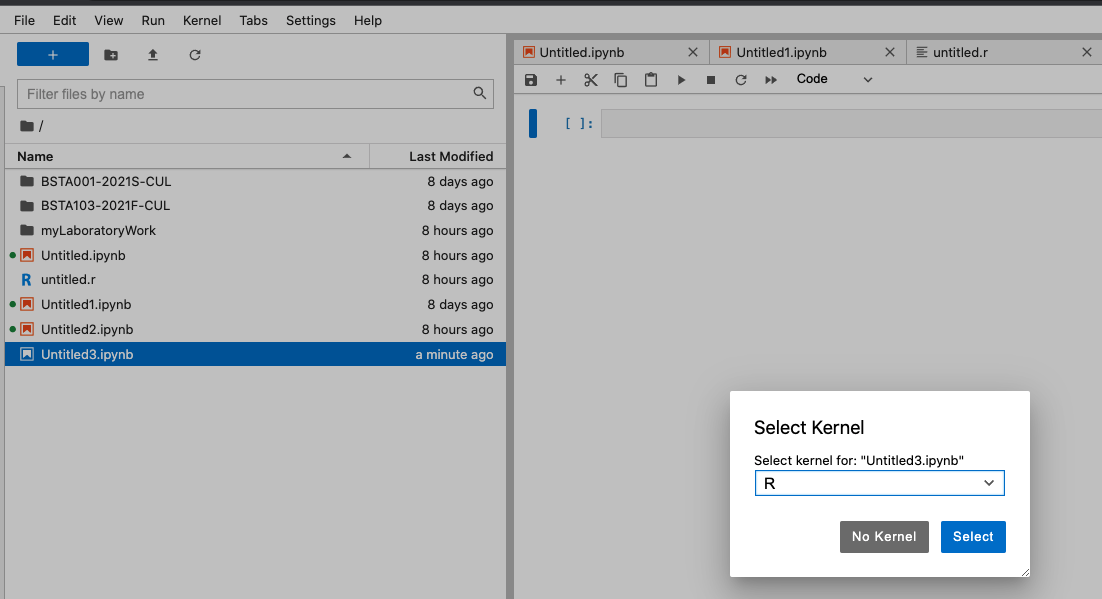
\includegraphics{chapters/chapter1/kernelselect}
\caption{kernelselect.png}
\end{figure}

\hypertarget{the-notebook}{%
\subsubsection{The notebook}\label{the-notebook}}

A notebook is a collection of cells. A \textbf{cell} is a container that
can hold text or computer code. Cells in Jupyter looks like gray
rectangles. There are three cell types in Jupyter: (i) Code, (ii)
Markdown, and (iii) Raw. The two that we will focus on are Code and
Markdown.

The ``Code'' cell holds computer code that the R kernel (see below about
a kernel) can use to compute. We may want to import data, run a
statistical analysis, and output results. This is for the ``Code'' cell.

``Markdown'' is itself a special language that a Jupyter Notebook
interprets as text. The ``Markdown'' cell is most useful for write ups,
descriptions of a Code cell above or below, or scientific conclusions,
comments, and thoughts. When you need to write, think Markdown.

\hypertarget{save-your-work}{%
\subsubsection{Save your work}\label{save-your-work}}

You can always save your work, and should do so often, by clicking File
-\textgreater{} Save Notebook.

\hypertarget{export-for-submission}{%
\subsubsection{Export for submission}\label{export-for-submission}}

In class, we will ask that you submit your work on Coursesite as a
\textbf{PDF}. Work in another format will not be accepted. To export
your notebook as a PDF, choose File-\textgreater Save and Export
Notebook As-\textgreater PDF 

\begin{figure}
    \centering
    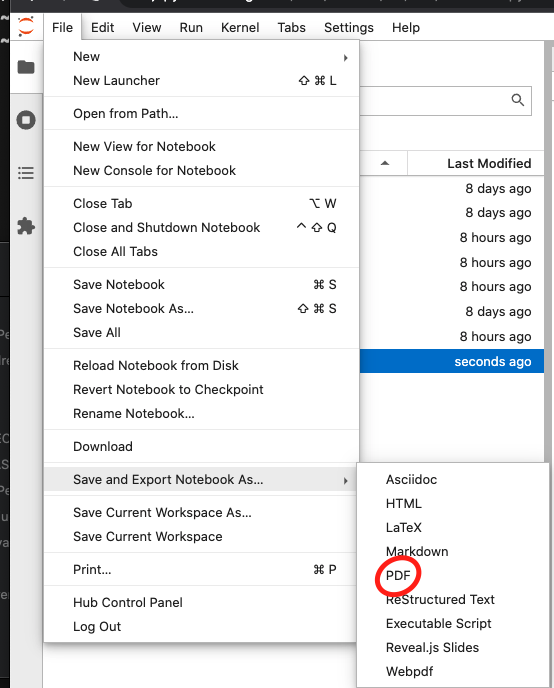
\includegraphics{chapters/chapter1/savepdf.png}
    \caption{Caption}
    \label{fig:my_label}
\end{figure}


After you
click PDF, a PDF file will be created and saved in a ``Downloads''
folder on your local machine. Make sure the PDF file contains (1) Your
first and surname, the date, and a descriptive title.

\hypertarget{kernel}{%
\subsection{Kernel}\label{kernel}}

The kernel is the component that executes code inside your notebook. No
kernel, no running code.

Over the course, you may find that your notebook has disconnected or
otherwise will no longer execute the code you wrote. Most often, the
kernel has stopped. To restart you kernel select
Kernel-\textgreater Restart Kernel.

    \hypertarget{programming-and-r}{%
\section{Programming and R}\label{programming-and-r}}

The R programming language, while not explictly written for statistics,
has a long history as a tool for data analysis, statistics, machine
learning, and data science. R supports all of the main paradigms in
computing and you will be able to transfer what you learn in R to other
programming languages without much difficulty.

Programming is difficult. Like any skill, programming take time to
master. Error messages will be commonplace, you will find it difficult
to ask the computer to calculate what you want. You will be frustrate
and that is ok. Over time you will learn to read the error messages,
code will flow more easily. The most important part of programming is
daily practice.

When we \textbf{execute} code, we ask the computer to translate what we
wrote into binary and return a set of results that may or may not be
stored in memory. In the Jupyter environment we execute code by pressing
``Run'' or by using the shortcut ``Shift+Enter''.

    \hypertarget{arithmetic}{%
\section{Arithmetic}\label{arithmetic}}

R supports all standard artithmetic calculations. Lets ``Run'' our first
computation.

R can interpret addition

    \begin{tcolorbox}[breakable, size=fbox, boxrule=1pt, pad at break*=1mm,colback=cellbackground, colframe=cellborder]
\prompt{In}{incolor}{100}{\boxspacing}
\begin{Verbatim}[commandchars=\\\{\}]
\PY{l+m}{2}\PY{l+m}{+2}
\end{Verbatim}
\end{tcolorbox}

    4

    
    Subtraction

    \begin{tcolorbox}[breakable, size=fbox, boxrule=1pt, pad at break*=1mm,colback=cellbackground, colframe=cellborder]
\prompt{In}{incolor}{101}{\boxspacing}
\begin{Verbatim}[commandchars=\\\{\}]
\PY{l+m}{9}\PY{l+m}{\PYZhy{}3}
\end{Verbatim}
\end{tcolorbox}

    6

    
    Division

    \begin{tcolorbox}[breakable, size=fbox, boxrule=1pt, pad at break*=1mm,colback=cellbackground, colframe=cellborder]
\prompt{In}{incolor}{102}{\boxspacing}
\begin{Verbatim}[commandchars=\\\{\}]
\PY{l+m}{3}\PY{o}{/}\PY{l+m}{4}
\end{Verbatim}
\end{tcolorbox}

    0.75

    
    multiplication

    \begin{tcolorbox}[breakable, size=fbox, boxrule=1pt, pad at break*=1mm,colback=cellbackground, colframe=cellborder]
\prompt{In}{incolor}{103}{\boxspacing}
\begin{Verbatim}[commandchars=\\\{\}]
\PY{l+m}{4}\PY{o}{*}\PY{l+m}{4}
\end{Verbatim}
\end{tcolorbox}

    16

    
    and exponentiation

    \begin{tcolorbox}[breakable, size=fbox, boxrule=1pt, pad at break*=1mm,colback=cellbackground, colframe=cellborder]
\prompt{In}{incolor}{104}{\boxspacing}
\begin{Verbatim}[commandchars=\\\{\}]
\PY{l+m}{3}\PY{o}{\PYZca{}}\PY{l+m}{9}
\end{Verbatim}
\end{tcolorbox}

    19683

    
    As expected, we can compute more difficult arithemetic expressions.

    \begin{tcolorbox}[breakable, size=fbox, boxrule=1pt, pad at break*=1mm,colback=cellbackground, colframe=cellborder]
\prompt{In}{incolor}{105}{\boxspacing}
\begin{Verbatim}[commandchars=\\\{\}]
\PY{p}{(}\PY{l+m}{2}\PY{o}{\PYZca{}}\PY{l+m}{4}\PY{p}{)}\PY{l+m}{+3}\PY{o}{/}\PY{l+m}{2} \PY{o}{\PYZhy{}} \PY{l+m}{1}
\end{Verbatim}
\end{tcolorbox}

    16.5

    
    \hypertarget{vectors}{%
\section{Vectors}\label{vectors}}

The \textbf{vector} is the fundemental object in R.

A mathematical vector is an ordered list of numbers. They are denoted by
a sequence of numbers surrounded by square brackets.

\begin{align}
    v = \begin{bmatrix}
         1 \\
         2 \\
         3 \\
        \end{bmatrix}
\end{align} Above, the vector \textbf{v} is a vector of length 3 and
contains, in order, the values 1, 2, and 3.

In R, vectors are goven a name and stored in the computer in one of two
ways: (i) using the \textbf{c()} operator or (ii) using the assign
function.

\hypertarget{assignment}{%
\subsection{Assignment}\label{assignment}}

\hypertarget{c}{%
\subsubsection{c()}\label{c}}

We can store a vector named v with the values 1,2,3 in R as follows

    \begin{tcolorbox}[breakable, size=fbox, boxrule=1pt, pad at break*=1mm,colback=cellbackground, colframe=cellborder]
\prompt{In}{incolor}{106}{\boxspacing}
\begin{Verbatim}[commandchars=\\\{\}]
\PY{n}{v} \PY{o}{=} \PY{n+nf}{c}\PY{p}{(}\PY{l+m}{1}\PY{p}{,}\PY{l+m}{2}\PY{p}{,}\PY{l+m}{3}\PY{p}{)}
\end{Verbatim}
\end{tcolorbox}

    \hypertarget{assign}{%
\subsubsection{assign}\label{assign}}

We can also use the assign function to store a vector, named q, with the
values 3,2,1 as follows

    \begin{tcolorbox}[breakable, size=fbox, boxrule=1pt, pad at break*=1mm,colback=cellbackground, colframe=cellborder]
\prompt{In}{incolor}{107}{\boxspacing}
\begin{Verbatim}[commandchars=\\\{\}]
\PY{n+nf}{assign}\PY{p}{(}\PY{l+s}{\PYZdq{}}\PY{l+s}{q\PYZdq{}}\PY{p}{,}\PY{n+nf}{c}\PY{p}{(}\PY{l+m}{3}\PY{p}{,}\PY{l+m}{2}\PY{p}{,}\PY{l+m}{1}\PY{p}{)}\PY{p}{)}
\end{Verbatim}
\end{tcolorbox}

    \hypertarget{equals}{%
\subsubsection{equals}\label{equals}}

The equals sign \textbf{does not} represent two objects are equal to one
another. The equals sign in compiuter programming stands for ``assign''.

When we write \texttt{v\ =\ c(1,2,3)}, this is understood as ``we assign
the variable v to the vector (1,2,3). As an example, lets create a
vector \texttt{(4,5,6)} names \texttt{x} and then assign the variable
\texttt{y} to be the same as \texttt{x}

    \begin{tcolorbox}[breakable, size=fbox, boxrule=1pt, pad at break*=1mm,colback=cellbackground, colframe=cellborder]
\prompt{In}{incolor}{108}{\boxspacing}
\begin{Verbatim}[commandchars=\\\{\}]
\PY{n}{x} \PY{o}{=} \PY{n+nf}{c}\PY{p}{(}\PY{l+m}{4}\PY{p}{,}\PY{l+m}{5}\PY{p}{,}\PY{l+m}{6}\PY{p}{)}
\PY{n}{y} \PY{o}{=} \PY{n}{x}
\end{Verbatim}
\end{tcolorbox}

    The last line above does not ask whether or not \texttt{x} is the same
as \texttt{y}. Instead, this line assigns the variable \texttt{y} to be
the same vecor as \texttt{x}.

    \hypertarget{print}{%
\section{Print}\label{print}}

When we created the vectors \textbf{v} and \textbf{q} ``nothing
happened''. Though the vector v and q were created and stored in the
computer, R does not display these on your screen by default. One way to
view any object in R is to print it.

You can print an object, \texttt{x}, R by writing \texttt{print(x)}

    \begin{tcolorbox}[breakable, size=fbox, boxrule=1pt, pad at break*=1mm,colback=cellbackground, colframe=cellborder]
\prompt{In}{incolor}{109}{\boxspacing}
\begin{Verbatim}[commandchars=\\\{\}]
\PY{n+nf}{print}\PY{p}{(}\PY{n}{v}\PY{p}{)}
\end{Verbatim}
\end{tcolorbox}

    \begin{Verbatim}[commandchars=\\\{\}]
[1] 1 2 3
    \end{Verbatim}

    \begin{tcolorbox}[breakable, size=fbox, boxrule=1pt, pad at break*=1mm,colback=cellbackground, colframe=cellborder]
\prompt{In}{incolor}{110}{\boxspacing}
\begin{Verbatim}[commandchars=\\\{\}]
\PY{n+nf}{print}\PY{p}{(}\PY{n}{q}\PY{p}{)}
\end{Verbatim}
\end{tcolorbox}

    \begin{Verbatim}[commandchars=\\\{\}]
[1] 3 2 1
    \end{Verbatim}

    \begin{tcolorbox}[breakable, size=fbox, boxrule=1pt, pad at break*=1mm,colback=cellbackground, colframe=cellborder]
\prompt{In}{incolor}{111}{\boxspacing}
\begin{Verbatim}[commandchars=\\\{\}]
\PY{n+nf}{print}\PY{p}{(}\PY{n}{x}\PY{p}{)}
\PY{n+nf}{print}\PY{p}{(}\PY{n}{y}\PY{p}{)}
\end{Verbatim}
\end{tcolorbox}

    \begin{Verbatim}[commandchars=\\\{\}]
[1] 4 5 6
[1] 4 5 6
    \end{Verbatim}

    \textbf{You do not need to print any object, ever}. Printing is not
necessary. You should use print to explore whether you programmed
something write or to communicate scientific results.

    \hypertarget{combining-vectors}{%
\section{Combining vectors}\label{combining-vectors}}

We can append one vector to another in R by using the c() operator.
Suppose we wish to combine the two vectors \begin{align}
    x = \begin{bmatrix}
        1\\
        2\\
        3
        \end{bmatrix}; \;
    z = \begin{bmatrix}
        -1\\
        0.2\\
        90
        \end{bmatrix}
\end{align}

into one vector

\begin{align}
    r = \begin{bmatrix}
        1\\
        2\\
        3\\
        -1\\
        0.2\\
        90
        \end{bmatrix}
\end{align}

Lets first create the vectors \texttt{x} and \texttt{z}

    \begin{tcolorbox}[breakable, size=fbox, boxrule=1pt, pad at break*=1mm,colback=cellbackground, colframe=cellborder]
\prompt{In}{incolor}{112}{\boxspacing}
\begin{Verbatim}[commandchars=\\\{\}]
\PY{n}{x} \PY{o}{=} \PY{n+nf}{c}\PY{p}{(}\PY{l+m}{1}\PY{p}{,}\PY{l+m}{2}\PY{p}{,}\PY{l+m}{3}\PY{p}{)}
\PY{n}{z} \PY{o}{=} \PY{n+nf}{c}\PY{p}{(}\PY{l+m}{\PYZhy{}1}\PY{p}{,}\PY{l+m}{0.2}\PY{p}{,}\PY{l+m}{90}\PY{p}{)}
\end{Verbatim}
\end{tcolorbox}

    Now we can create the vector \texttt{r}

    \begin{tcolorbox}[breakable, size=fbox, boxrule=1pt, pad at break*=1mm,colback=cellbackground, colframe=cellborder]
\prompt{In}{incolor}{113}{\boxspacing}
\begin{Verbatim}[commandchars=\\\{\}]
\PY{n}{r} \PY{o}{=} \PY{n+nf}{c}\PY{p}{(}\PY{n}{x}\PY{p}{,}\PY{n}{z}\PY{p}{)}
\end{Verbatim}
\end{tcolorbox}

    If we want to check our work, we can print out \texttt{r}.

    \begin{tcolorbox}[breakable, size=fbox, boxrule=1pt, pad at break*=1mm,colback=cellbackground, colframe=cellborder]
\prompt{In}{incolor}{114}{\boxspacing}
\begin{Verbatim}[commandchars=\\\{\}]
\PY{n+nf}{print}\PY{p}{(}\PY{n}{r}\PY{p}{)}
\end{Verbatim}
\end{tcolorbox}

    \begin{Verbatim}[commandchars=\\\{\}]
[1]  1.0  2.0  3.0 -1.0  0.2 90.0
    \end{Verbatim}

    \hypertarget{indexing-and-access}{%
\section{Indexing and access}\label{indexing-and-access}}

Vectors are useful for storing several different numbers. We can access
single elements, or several elements inside a vector by (i) naming the
vector we want to access, (ii) typing square brackets ``{[}{]}''.

\hypertarget{numeric-indexing}{%
\subsection{Numeric indexing}\label{numeric-indexing}}

If we want to access the 4th element in \texttt{r}, we can type

    \begin{tcolorbox}[breakable, size=fbox, boxrule=1pt, pad at break*=1mm,colback=cellbackground, colframe=cellborder]
\prompt{In}{incolor}{115}{\boxspacing}
\begin{Verbatim}[commandchars=\\\{\}]
\PY{n}{r}\PY{p}{[}\PY{l+m}{4}\PY{p}{]}
\end{Verbatim}
\end{tcolorbox}

    -1

    
    If we want to access, the 2nd, 4th, and then the first element of
\texttt{r} we can include in square brackets the vector
\texttt{c(2,4,1)}

    \begin{tcolorbox}[breakable, size=fbox, boxrule=1pt, pad at break*=1mm,colback=cellbackground, colframe=cellborder]
\prompt{In}{incolor}{116}{\boxspacing}
\begin{Verbatim}[commandchars=\\\{\}]
\PY{n}{r}\PY{p}{[}\PY{n+nf}{c}\PY{p}{(}\PY{l+m}{2}\PY{p}{,}\PY{l+m}{4}\PY{p}{,}\PY{l+m}{1}\PY{p}{)}\PY{p}{]}
\end{Verbatim}
\end{tcolorbox}

    \begin{enumerate*}
\item 2
\item -1
\item 1
\end{enumerate*}


    
    We can access the 1st,2nd, and 3rd elements in \texttt{r} using the
vector \texttt{c(1,2,3)}, however a shortcut is to use the
\textbf{colon} operator. The colon operator takes as input two integers
(a,b) separated by a colon (a:b) and expands to the vector
\texttt{c(a,a+1,a+2,a+3,...,b)}.

Watch

    \begin{tcolorbox}[breakable, size=fbox, boxrule=1pt, pad at break*=1mm,colback=cellbackground, colframe=cellborder]
\prompt{In}{incolor}{117}{\boxspacing}
\begin{Verbatim}[commandchars=\\\{\}]
\PY{n}{z} \PY{o}{=} \PY{l+m}{3}\PY{o}{:}\PY{l+m}{5}
\end{Verbatim}
\end{tcolorbox}

    \begin{tcolorbox}[breakable, size=fbox, boxrule=1pt, pad at break*=1mm,colback=cellbackground, colframe=cellborder]
\prompt{In}{incolor}{118}{\boxspacing}
\begin{Verbatim}[commandchars=\\\{\}]
\PY{n+nf}{print}\PY{p}{(}\PY{n}{z}\PY{p}{)}
\end{Verbatim}
\end{tcolorbox}

    \begin{Verbatim}[commandchars=\\\{\}]
[1] 3 4 5
    \end{Verbatim}

    The colon operator is useful for accessing items in a vector

    \begin{tcolorbox}[breakable, size=fbox, boxrule=1pt, pad at break*=1mm,colback=cellbackground, colframe=cellborder]
\prompt{In}{incolor}{119}{\boxspacing}
\begin{Verbatim}[commandchars=\\\{\}]
\PY{n}{r}\PY{p}{[}\PY{l+m}{2}\PY{o}{:}\PY{l+m}{5}\PY{p}{]}
\end{Verbatim}
\end{tcolorbox}

    \begin{enumerate*}
\item 2
\item 3
\item -1
\item 0.2
\end{enumerate*}


    
    The above is called \textbf{numeric indexing}. Numeric indexing is the
access of elements in an object (here a vector) by inputting a single
number, or vector of numbers. Indices are always integers. Fractional or
decimal numbers cannot be used as indices. Up until now we only used
\emph{positive} integers to access elements of a vector.

R also accepts negative integers as indices. Warning: R handles negative
indices different than the majority of other progamming languages. A
negative index in R standard for \textbf{exclude}.

For example, if we want to return all the elements of a vector
\texttt{q\ =\ c(1,4,6,10,0.5)} except for the 2nd element, we can write
\texttt{q{[}-2{]}}

    \begin{tcolorbox}[breakable, size=fbox, boxrule=1pt, pad at break*=1mm,colback=cellbackground, colframe=cellborder]
\prompt{In}{incolor}{120}{\boxspacing}
\begin{Verbatim}[commandchars=\\\{\}]
\PY{n}{q} \PY{o}{=} \PY{n+nf}{c}\PY{p}{(}\PY{l+m}{1}\PY{p}{,}\PY{l+m}{4}\PY{p}{,}\PY{l+m}{6}\PY{p}{,}\PY{l+m}{10}\PY{p}{,}\PY{l+m}{0.5}\PY{p}{)}
\PY{n}{q}\PY{p}{[}\PY{l+m}{\PYZhy{}2}\PY{p}{]}
\end{Verbatim}
\end{tcolorbox}

    \begin{enumerate*}
\item 1
\item 6
\item 10
\item 0.5
\end{enumerate*}


    
    \hypertarget{logical-vectors-and-logical-indexing}{%
\subsection{Logical vectors and logical
indexing}\label{logical-vectors-and-logical-indexing}}

\hypertarget{true-and-false}{%
\subsubsection{True and False}\label{true-and-false}}

R, like all programming languages, understands how to operate with
binary logic (aside: binary logic is not the only type. If interested,
google the tetralemma). True in R is represeted as the word
\texttt{TRUE} in all capitals. False in R is represented as the word
\texttt{FALSE} in all capitals. The symbols \texttt{TRUE} and
\texttt{FALSE} are reserved, special symbols in R. You cannot assign a
variable to \texttt{TRUE} or \texttt{FALSE}.

    \begin{tcolorbox}[breakable, size=fbox, boxrule=1pt, pad at break*=1mm,colback=cellbackground, colframe=cellborder]
\prompt{In}{incolor}{121}{\boxspacing}
\begin{Verbatim}[commandchars=\\\{\}]
\PY{k+kc}{TRUE}
\end{Verbatim}
\end{tcolorbox}

    TRUE

    
    \begin{tcolorbox}[breakable, size=fbox, boxrule=1pt, pad at break*=1mm,colback=cellbackground, colframe=cellborder]
\prompt{In}{incolor}{122}{\boxspacing}
\begin{Verbatim}[commandchars=\\\{\}]
\PY{k+kc}{FALSE}
\end{Verbatim}
\end{tcolorbox}

    FALSE

    
    \hypertarget{logical-comparisons}{%
\subsubsection{Logical comparisons}\label{logical-comparisons}}

R understand the following logical operators: - \texttt{\textgreater{}}
``Greater than'' - \texttt{\textgreater{}=} ``Greater than or equal to''
- \texttt{\textless{}} ``Less than'' - \texttt{\textless{}=} ``Less than
or equal to'' - \texttt{==} ``Is equal to'' - \texttt{!=} ``Not equal''
- \texttt{\textbar{}} ``OR'' - \texttt{\&} ``AND''

\hypertarget{logic}{%
\subsubsection{Logic}\label{logic}}

Logic is a method to evaluate statements, sometimes called propositions
as either True or False. The above symbols are used to evaluate
statements.

When you pose a proposition to R, such as \texttt{v\ \textgreater{}\ -1}
R will evaluate that propositon for each individual element in the
vector \texttt{v}. Lets create the vector \texttt{v\ =\ c(-10,10,4)} and
ask R to evaluate the proposition \texttt{v\textgreater{}-1}.

    \begin{tcolorbox}[breakable, size=fbox, boxrule=1pt, pad at break*=1mm,colback=cellbackground, colframe=cellborder]
\prompt{In}{incolor}{123}{\boxspacing}
\begin{Verbatim}[commandchars=\\\{\}]
\PY{n}{v} \PY{o}{=} \PY{n+nf}{c}\PY{p}{(}\PY{l+m}{\PYZhy{}10}\PY{p}{,}\PY{l+m}{10}\PY{p}{,}\PY{l+m}{4}\PY{p}{)}
\PY{n}{v} \PY{o}{\PYZgt{}} \PY{l+m}{\PYZhy{}1}
\end{Verbatim}
\end{tcolorbox}

    \begin{enumerate*}
\item FALSE
\item TRUE
\item TRUE
\end{enumerate*}


    
    We see that R returns a vector with the same numebr of elements as in v
containing the values TRUE or FALSE. A vector that contains values
TRUE/FALSE is called a \textbf{logical vector}. Like any other vector we
can store a logical vector.

    \begin{tcolorbox}[breakable, size=fbox, boxrule=1pt, pad at break*=1mm,colback=cellbackground, colframe=cellborder]
\prompt{In}{incolor}{124}{\boxspacing}
\begin{Verbatim}[commandchars=\\\{\}]
\PY{n}{log} \PY{o}{=} \PY{n}{v}\PY{o}{\PYZgt{}}\PY{l+m}{\PYZhy{}1}
\end{Verbatim}
\end{tcolorbox}

    \begin{tcolorbox}[breakable, size=fbox, boxrule=1pt, pad at break*=1mm,colback=cellbackground, colframe=cellborder]
\prompt{In}{incolor}{125}{\boxspacing}
\begin{Verbatim}[commandchars=\\\{\}]
\PY{n+nf}{print}\PY{p}{(}\PY{n}{log}\PY{p}{)}
\end{Verbatim}
\end{tcolorbox}

    \begin{Verbatim}[commandchars=\\\{\}]
[1] FALSE  TRUE  TRUE
    \end{Verbatim}

    \hypertarget{and-or-and-not}{%
\subsubsection{AND, OR, and NOT}\label{and-or-and-not}}

AND, OR, and NOT are \textbf{logical operators}, they allow us to
combine one or more propositions. Given two propositions \(p_{1}\) and
\(p_{2}\), the AND, OR, and NOT operator will evaluate to the following


\begin{table}[ht!]
    \centering
    \begin{tabular}{ccccc}
        \hline
        $p_{1}$ &$p_{2}$ &$p_{1}$ AND $p_{2}$ &$p_{1}$ OR $p_{2}$ &!$p_{1}$\\
        \hline \vspace{1mm}
        TRUE & TRUE & TRUE & TRUE & FALSE \\
        TRUE & FALSE & FALSE & TRUE & FALSE \\
        FALSE & TRUE & FALSE & TRUE & TRUE \\
        FALSE & FALSE & FALSE & FALSE & TRUE \\
    \hline
    \end{tabular}
    \caption{Caption}
    \label{tab:my_label}
\end{table}


Logical operators come in handy in \textbf{logical indexing}. When we
write \texttt{r{[}l{]}} where \texttt{l} is a logical vector, R will
return the the values in \texttt{r} where \texttt{l} is TRUE.

    \begin{tcolorbox}[breakable, size=fbox, boxrule=1pt, pad at break*=1mm,colback=cellbackground, colframe=cellborder]
\prompt{In}{incolor}{126}{\boxspacing}
\begin{Verbatim}[commandchars=\\\{\}]
\PY{n}{r} \PY{o}{=} \PY{n+nf}{c}\PY{p}{(}\PY{l+m}{\PYZhy{}10}\PY{p}{,}\PY{l+m}{0}\PY{p}{,}\PY{l+m}{10}\PY{p}{,}\PY{l+m}{55}\PY{p}{,}\PY{l+m}{0.34}\PY{p}{,}\PY{l+m}{\PYZhy{}0.97}\PY{p}{)}
\PY{n}{l} \PY{o}{=} \PY{n+nf}{c}\PY{p}{(}\PY{k+kc}{TRUE}\PY{p}{,}\PY{k+kc}{FALSE}\PY{p}{,}\PY{k+kc}{TRUE}\PY{p}{,}\PY{k+kc}{FALSE}\PY{p}{,}\PY{k+kc}{TRUE}\PY{p}{,}\PY{k+kc}{TRUE}\PY{p}{)}

\PY{n}{r}\PY{p}{[}\PY{n}{l}\PY{p}{]}
\end{Verbatim}
\end{tcolorbox}

    \begin{enumerate*}
\item -10
\item 10
\item 0.34
\item -0.97
\end{enumerate*}


    
    More often we will include the logical statement directly inside the
square brackets

    \begin{tcolorbox}[breakable, size=fbox, boxrule=1pt, pad at break*=1mm,colback=cellbackground, colframe=cellborder]
\prompt{In}{incolor}{127}{\boxspacing}
\begin{Verbatim}[commandchars=\\\{\}]
\PY{n}{r}\PY{p}{[} \PY{n}{r}\PY{o}{\PYZgt{}}\PY{l+m}{0} \PY{p}{]}
\end{Verbatim}
\end{tcolorbox}

    \begin{enumerate*}
\item 10
\item 55
\item 0.34
\end{enumerate*}


    
    \hypertarget{equivalence-of-true-and-false-to-1-and-0}{%
\subsubsection{Equivalence of TRUE and FALSE to 1 and
0}\label{equivalence-of-true-and-false-to-1-and-0}}

    The symbol \texttt{TRUE} in R is understood to be the same as the value
\texttt{1}, and the symbol \texttt{FALSE} in R is understood to be the
same value as \texttt{0}.

    \begin{tcolorbox}[breakable, size=fbox, boxrule=1pt, pad at break*=1mm,colback=cellbackground, colframe=cellborder]
\prompt{In}{incolor}{128}{\boxspacing}
\begin{Verbatim}[commandchars=\\\{\}]
\PY{k+kc}{TRUE}\PY{o}{==}\PY{l+m}{1}
\end{Verbatim}
\end{tcolorbox}

    TRUE

    
    \begin{tcolorbox}[breakable, size=fbox, boxrule=1pt, pad at break*=1mm,colback=cellbackground, colframe=cellborder]
\prompt{In}{incolor}{129}{\boxspacing}
\begin{Verbatim}[commandchars=\\\{\}]
\PY{k+kc}{FALSE}\PY{o}{==}\PY{l+m}{0}
\end{Verbatim}
\end{tcolorbox}

    TRUE

    
    \begin{tcolorbox}[breakable, size=fbox, boxrule=1pt, pad at break*=1mm,colback=cellbackground, colframe=cellborder]
\prompt{In}{incolor}{130}{\boxspacing}
\begin{Verbatim}[commandchars=\\\{\}]
\PY{k+kc}{TRUE}\PY{o}{==}\PY{l+m}{0}
\end{Verbatim}
\end{tcolorbox}

    FALSE

    
    \begin{tcolorbox}[breakable, size=fbox, boxrule=1pt, pad at break*=1mm,colback=cellbackground, colframe=cellborder]
\prompt{In}{incolor}{131}{\boxspacing}
\begin{Verbatim}[commandchars=\\\{\}]
\PY{k+kc}{FALSE}\PY{o}{==}\PY{l+m}{1}
\end{Verbatim}
\end{tcolorbox}

    FALSE

    
    \hypertarget{two-functions-that-are-useul-for-operating-on-vectors}{%
\subsection{Two functions that are useul for operating on
vectors}\label{two-functions-that-are-useul-for-operating-on-vectors}}

Functions in mathematics take as input a list of objects and return a
unique object. The same is true of functions in programming and so in R.

We can create our own functions in R (this will come later), but R also
has a large library of built-in functions that are automatically
included once you start R. Two very sueful ones are the \texttt{sum}
function and the \texttt{length} function.

The \texttt{sum} function takes as input a vector and returns the sum of
each element in the function.

    \begin{tcolorbox}[breakable, size=fbox, boxrule=1pt, pad at break*=1mm,colback=cellbackground, colframe=cellborder]
\prompt{In}{incolor}{133}{\boxspacing}
\begin{Verbatim}[commandchars=\\\{\}]
\PY{n}{v} \PY{o}{=} \PY{n+nf}{c}\PY{p}{(}\PY{l+m}{3}\PY{p}{,}\PY{l+m}{2}\PY{p}{,}\PY{l+m}{1}\PY{p}{)}
\PY{n+nf}{sum}\PY{p}{(}\PY{n}{v}\PY{p}{)}
\end{Verbatim}
\end{tcolorbox}

    6

    
    The \texttt{length} function takes as input a vector and returns the
number of elements in the vector

    \begin{tcolorbox}[breakable, size=fbox, boxrule=1pt, pad at break*=1mm,colback=cellbackground, colframe=cellborder]
\prompt{In}{incolor}{134}{\boxspacing}
\begin{Verbatim}[commandchars=\\\{\}]
\PY{n+nf}{length}\PY{p}{(}\PY{n}{v}\PY{p}{)}
\end{Verbatim}
\end{tcolorbox}

    3

    
    \hypertarget{assignment-01}{%
\section{Assignment 01}\label{assignment-01}}

We are recruited to track the evolution of an infectious agent for a
team of public health officials (PHOs). To support future strategic
planning the PHOs want to know the impact of intervention \(X\) on
increases or decreases in the incidence of this infectious agent. The
PHO team collected for each county in their state whether the
intervention was enacted, and whether the incidence of case counts of
this infectious agent increased or decreased 60 days after the
intervention was in place data.

Using R, we will assign probabiltiies to the four events in our sample
space \{ (intervention,raise),(intervention, no raise),(no intervention,
raise),(no intervention, no raise) \}

\hypertarget{the-data}{%
\subsection{The data}\label{the-data}}

In the below cell there is a few lines of code pre-programmed. Please
runs this cell below.

This cell will create two vectors.

The first vector is called \texttt{intervention\_rise} and contains one
element for each county that has intervention \(X\) collected by the PHO
team. An element is the value \texttt{1} if there was a rise in
incidence for the infectious agent and \texttt{0} if there was a fall in
incidence.

The second vector is called \texttt{nointervention\_rise} and contains
one element for each county that did not have intervention \(X\)
collected by the PHO team. An element is the value \texttt{1} if there
was a rise in incidence for the infectious agent and \texttt{0} if there
was a fall in incidence.

\hypertarget{please-complete-the-following}{%
\subsection{Please complete the
following}\label{please-complete-the-following}}

\begin{enumerate}
\def\labelenumi{\arabic{enumi}.}
\tightlist
\item
  Use the \texttt{length} function to count the number of counties where
  intervention \(X\) took place
\item
  Use the \texttt{length} function to count the number of counties where
  no intervention \(X\) took place
\item
  Use the \texttt{sum} function to count the number of counties that
  observed a rise in incidence.
\item
  Use the \texttt{sum} function and the \texttt{not\ (!)} operator to
  count the number of counties that observed a fall in incidence.
\item
  Use the frequentist approach to compute the probability

  \begin{itemize}
  \tightlist
  \item
    that an intervention would take place in a county
  \item
    that a rise in incidence was observed in a county
  \item
    of a rise in incidence given a county implemented intervention \(X\)
  \item
    of a rise in incidence given a county has not implemented
    intervention \(X\)
  \end{itemize}
\item
  Use the multiplication rule to compute the probability

  \begin{itemize}
  \tightlist
  \item
    that an intervention and rise is observed (Hint: P(Intervention) *
    P(Rise\textbar Intervention))
  \item
    that an intervention and fall is observed
  \item
    that no intervention and rise is observed
  \item
    that no intervention and fall is observed
  \end{itemize}
\item
  Compute the probability of the below events, assuming intervention and
  rise/fall. are independent

  \begin{itemize}
  \tightlist
  \item
    Intervention and Rise
  \item
    Intervention and Fall
  \item
    No Intervention and Rise\\
  \item
    No Intervention and Fall
  \end{itemize}
\item
  Do you think intervention \(X\) is effective at preventing the spread
  of our infectious agent?
\end{enumerate}

    \begin{tcolorbox}[breakable, size=fbox, boxrule=1pt, pad at break*=1mm,colback=cellbackground, colframe=cellborder]
\prompt{In}{incolor}{178}{\boxspacing}
\begin{Verbatim}[commandchars=\\\{\}]
\PY{c+c1}{\PYZsh{}RUN THIS CODE. DO NOT WORRY WHAT IT SAYS. }
\PY{n}{nums} \PY{o}{=} \PY{n+nf}{runif}\PY{p}{(}\PY{l+m}{10}\PY{o}{\PYZca{}}\PY{l+m}{3}\PY{p}{,}\PY{l+m}{0}\PY{p}{,}\PY{l+m}{1}\PY{p}{)}

\PY{n}{intervention\PYZus{}rise}   \PY{o}{=} \PY{n+nf}{c}\PY{p}{(}\PY{p}{)}
\PY{n}{nointervention\PYZus{}rise} \PY{o}{=} \PY{n+nf}{c}\PY{p}{(}\PY{p}{)}
\PY{n+nf}{for }\PY{p}{(}\PY{n}{i} \PY{n}{in} \PY{n}{nums}\PY{p}{)}\PY{p}{\PYZob{}}
    \PY{n+nf}{if }\PY{p}{(}\PY{n+nf}{runif}\PY{p}{(}\PY{l+m}{1}\PY{p}{)}\PY{o}{\PYZgt{}} \PY{l+m}{0.4}\PY{p}{)}\PY{p}{\PYZob{}}
        \PY{n+nf}{if }\PY{p}{(} \PY{n}{i}\PY{o}{\PYZgt{}}\PY{l+m}{0.800} \PY{p}{)}\PY{p}{\PYZob{}}
          \PY{n}{risefall} \PY{o}{=} \PY{l+m}{1}   
        \PY{p}{\PYZcb{}} \PY{n}{else}\PY{p}{\PYZob{}}\PY{n}{risefall}\PY{o}{=}\PY{l+m}{0}\PY{p}{\PYZcb{}}
        \PY{n}{intervention\PYZus{}rise} \PY{o}{=} \PY{n+nf}{c}\PY{p}{(}\PY{n}{intervention\PYZus{}rise}\PY{p}{,} \PY{n}{risefall}\PY{p}{)}
    \PY{p}{\PYZcb{}}
    \PY{n}{else} \PY{p}{\PYZob{}}
        \PY{n+nf}{if }\PY{p}{(} \PY{n}{i}\PY{o}{\PYZgt{}}\PY{l+m}{0.325} \PY{p}{)}\PY{p}{\PYZob{}}
          \PY{n}{risefall} \PY{o}{=} \PY{l+m}{1}   
        \PY{p}{\PYZcb{}} \PY{n}{else}\PY{p}{\PYZob{}}\PY{n}{risefall}\PY{o}{=}\PY{l+m}{0}\PY{p}{\PYZcb{}}
        \PY{n}{nointervention\PYZus{}rise} \PY{o}{=} \PY{n+nf}{c}\PY{p}{(}\PY{n}{nointervention\PYZus{}rise}\PY{p}{,} \PY{n}{risefall}\PY{p}{)}
    \PY{p}{\PYZcb{}}
\PY{p}{\PYZcb{}}
\end{Verbatim}
\end{tcolorbox}
